

\section{Maps}
Maps were designed in a top-down view. The one limitation was that walls were perpendicular to floors and both floors and ceilings were horizontal so maps were drawn in 2D. A designer worked with five types of element: \cw{VERTEX}\footnote{Vertex coordinates were expressed with signed short integers [-32768, 32767]. 32 units translate to roughly one meter (or 3.28 feet for poor souls who must use the imperial system.)}, \cw{LINE}, \cw{SIDEDEF}, \cw{SECTOR}, and \cw{THING}.\\
\par
\drawing{doom_map_basics}{\doom{} map and the resulting data authored via DoomED}

\par
A \cw{SECTOR} is a closed area surrounded by \cw{LINE}s with a specified floor height, floor texture, ceiling height, ceiling texture, and light level. A sector can be concave, but lines cannot cross each other.\\
\par
A \cw{LINE} can either be a solid wall or a portal between two \cw{SECTOR}s. The difference is in the number of \cw{SIDEDEF}s associated with it. A wall has only one \cw{SIDEDEF} on its right side and is fully opaque. A portal has two \cw{SIDEDEF}s and can usually be partially seen though.\\
\par
A \cw{SIDEDEF} describes one side of a \cw{LINE}. To accommodate texturing of both the walls and portals, it can have up to three textures. The middle texture is used by walls for the full area they cover. A \cw{SIDEDEF} can also have a lower and an upper texture for portals connecting \cw{SECTOR}s with different ceiling/floor heights. If the portal leads to a sector with higher floor, the lower texture is used to render the "step". If the \cw{SECTOR} connects to a \cw{SECTOR} with a lower ceiling, the upper texture is used to render the "down step". To help alignment of doors and buttons, \cw{SIDEDEF} textures can have a vertical/horizontal offset. \\
\par
A \cw{THING} is much simpler in comparison. It only features a 2D-coordinate \cw{X,Y}, an angle, and an identifier controlling its type. At the bare minimum a map must have one player-spawning location \cw{THING}.\\

\cfullimage{doom_map.png}{Rendering of map shown in figure \ref{doom_map_basics}.}
\par

The resulting scene in figure \ref{doom_map.png} is ugly but the mismatched colors hopefully help to discern the different elements. All \cw{LINE}s are walls except for \cw{E-B} which has two \cw{SIDEDEF}s and is therefore a portal. All walls use the \cw{BRIK} middle texture except for the portal which uses \cw{GRAY} for both top and bottom.\\
\par
\cw{SECTOR} \#0 uses a \cw{RED} floor texture and a \cw{WOOD} ceiling texture. The height of the floor is 20 and its ceiling is at 40. \cw{SECTOR} \#1 uses a \cw{BLUE} floor texture and a \cw{GREEN} ceiling texture. Its floor is at 0 and ceiling at 60. Both sectors have the same light level (10).\\
\par
   Notice the portal \cw{E-B} which does not have a mid-texture but an upper and a lower texture. These were used to draw the up-step and down-step towards sector \#0.\\
\par
Also notice wall \cw{D-E} on which the mid-texture vertical offset is not correctly set, resulting in a vertical tear when connecting with wall \cw{E-F}. Wall \cw{B-C}'s vertical offset is properly set and has no visual artifact. None of the walls use a horizontal offset, but the corresponding field is labeled \cw{XOFF} on figure \ref{doom_map_basics} to show its location.\\ 
\pagebreak



\subsection{Map Editor (DoomED)}
To harness the complexity of the map format, a new tool was created to replace TED5\footnote{id Software map editor up to that point.}. The Doom map editor was to be called \textbf{DoomED}. This is where the \NeXT solution gave the most impact. The high resolution of the display allowed a lot of real-estate showing small details and many widgets. The stability of NeXTSTEP allowed one to never lose work while writing DoomED or creating a map.
The very design of Objective-C also had a tremendous influence. The language's message-dispatching system gracefully handled \cw{nullptr}\footnote{"Understanding the Objective-C Runtime" by Colin Wheeler.} dereferences, resulting in a fault-forgiving environment where a faulty feature would not work but did not crash either.\\
\par   
The killer feature was Interface Builder which not only came with a full library of widgets but also allowed creating new ones and connecting them to the business logic instantly.\\
\par
\fullimage{doomed/DoomEd.png}
\par

The release of the source code in April 2015 allowed programmers to peek inside. There is half as much code as in the game engine (doom:32kloc, DoomED:20kloc). Without the power of \NeXTns, the editor would have taken at least twice that amount of time to make.



\tcode{cloc_doomed.txt}
\par
DoomED was designed to be the "Adobe Illustrator for World Maps" where the designer simply drew lines, selected sectors, and picked textures.\\
\par
\vspace{10pt}
\trivia{DoomED's icon resembles a Baron of Hell. Upon startup an Imp growling sound is played.}\\
\par
\fullimage{doomed/all_widgets.png}\\
\par
DoomED did not output data usable by the game engine directly. Instead it generated a text format output called \cw{DWD}. A header served as a magic number which was followed by a list of lines (including sidedefs) and a list of things. Sectors were inferred from a line's ceiling/floor textures, ceiling/floor height, and light properties.\\
\par
\tcode{map.txt}
\par
DWD was not designed with space efficiency in mind but rather to be easy to parse since it was post-processed by the node builder tool, \cw{doombsp}.\\
\par
\cfullimage{props/tom.png}{Tom Hall, seemingly delighted, working on what would later be called E2M7. The sticker on his monitor reads, "quality".}
\par

\pagebreak





\section{Map Preprocessor (Node Builder)}
Map pre-processing was not something new at id. Since 1991 with Wolfenstein 3D, maps were already pre-processed to allow fast sound propagation. With \doom, it was taken to a whole new level both in terms of complexity and processing time.\\
\par
The main issue at hand was to maintain the same rendering speed despite relaxing the orthogonal grid constraints of Wolfenstein and losing the ability to use the DDA algorithm \footnote{Digital Differential Analyzer was used extensively for VSD (Visual Surface Determination), collision detection, and line-of-sight calculations. This was all gone with \doom.}. The solution chosen was to generate a multitude of accelerating data structures for each map, each dedicated to solving a particular problem.\\
\par
 The tool to do that was called \cw{doombsp}. It took as input a \cw{.DWD} map and outputted a \cw{.WAD}. Not only was the map expressed in a space-efficient format (e.g. expressing vertices only once and referencing them via index), but three data structures were generated alongside it. A binary space-partitioned version of the map expressed a node tree to speed up rendering. A blockmap accelerated collision detection. Finally, a reject table accelerated A.I. processing.\\
 \par
\trivia{Map preprocessing took a significant amount of time. With a NextStation TurboColor, running \cw{doombsp} on \cw{E1M1} took 10s. On E1M2, it took 30s. On E2M7, it took a full minute. The first nine maps of the shareware took 3m26s to process. The full twenty seven maps of the registered version requested 11 minutes.}\\% This was a problem for designers...yet it was little compared to what Quake's \cw{qbsp} would be three years later.}\\
\par
\tcode{cloc_doombsp.txt}
\par
 \trivia{\cw{DoomED.app}, \cw{doom} and \cw{doombsp} were tightly coupled. One button in the editor was enough to save the map, invoke the node builder and start the game with the WIP map.}


%
\begin{figure}[H]
\vspace*{3mm}
\centering
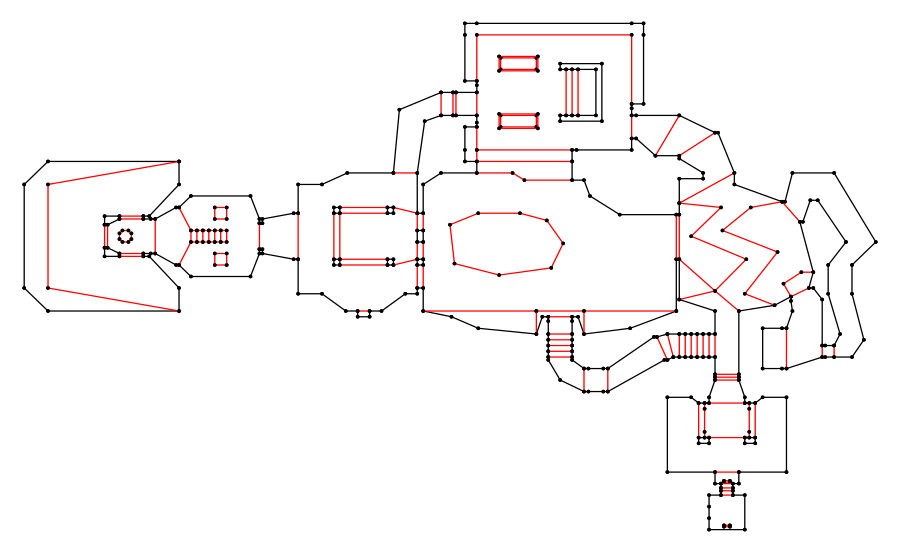
\includegraphics[width=\textwidth]{drawings/E1M1_lines.pdf}
\end{figure}
\par
The map as it is generated via DoomED. Portals are red. Walls are black.\\
\par
\begin{figure}[H]
\vspace*{2mm}
\centering
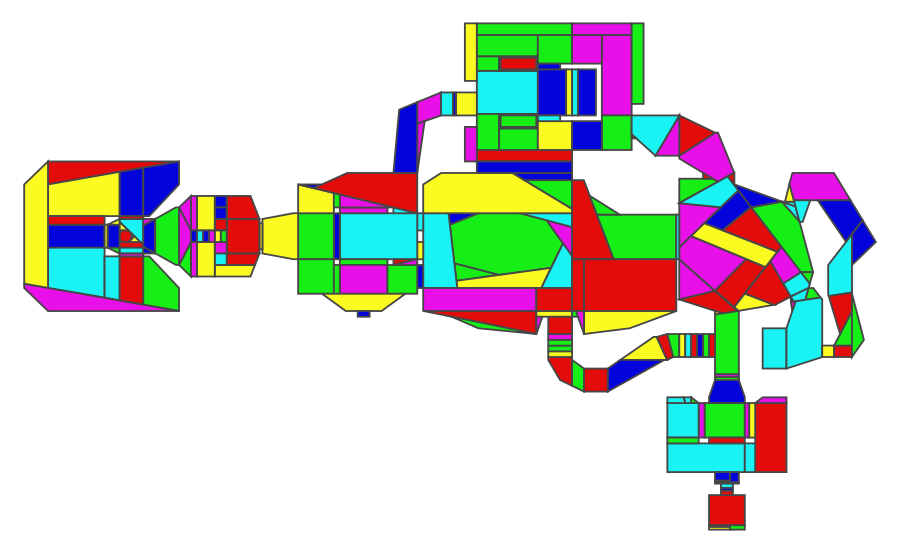
\includegraphics[width=\textwidth]{drawings/E1M1_fab.pdf}
\end{figure}
The BSP node tree where sectors are split into convex sub-spaces called sub-sectors.



\begin{figure}[H]
\centering
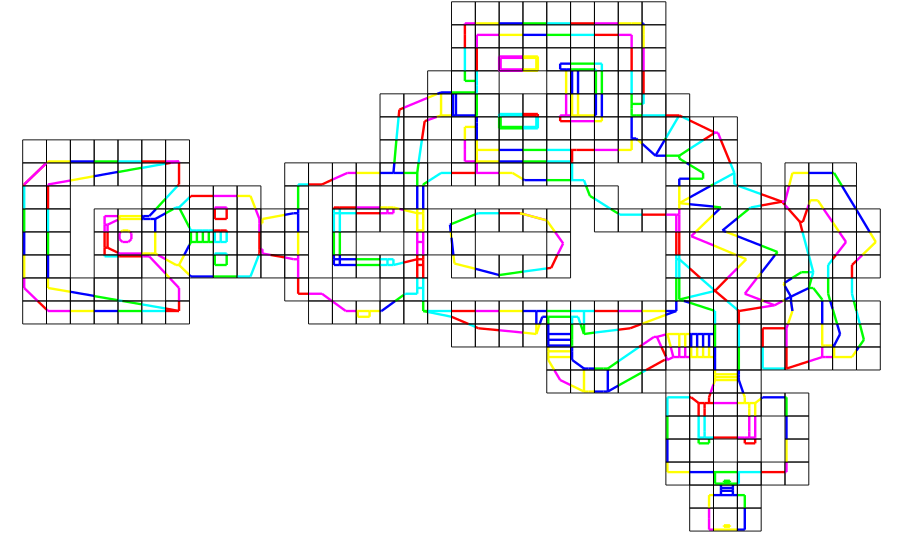
\includegraphics[width=\textwidth]{drawings/E1M1_blockmap.pdf}
\end{figure}
\par
Blockmap slicing where each block is 128x128 to accelerate collision detection.\\
\par
\begin{figure}[H]
\centering
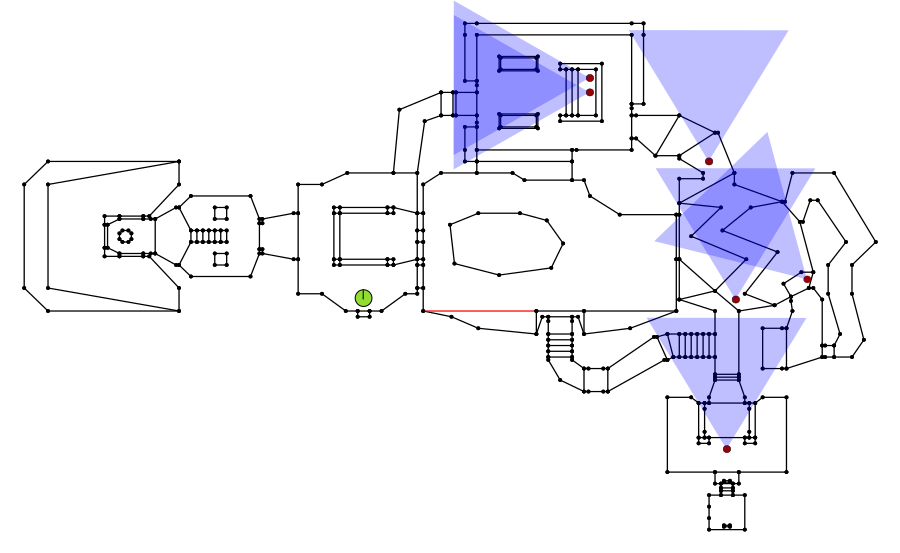
\includegraphics[width=\textwidth]{drawings/E1M1_sides_with_player.pdf}
\end{figure}
\par
The REJECT data structure to speed up enemies' and monsters' lines of sight calculations.
\pagebreak


The source code of the node builder was released shortly after the game in May 1994. It was the NeXTSTEP version but it was quickly converted to DOS and released under the name IDBSP to the delight of a hoard of modders.\\
\par
\cfullimage{doombsp_compiling.png}{Building doombsp on NeXTSTEP.}
\par
% \vspace{-10pt}
For each \cw{.dwd}, \cw{doombsp} outputs a set of lumps and stores them in a \cw{.wad} file (see p\pageref{wad_explained}).\\

\par
 \begin{figure}[H]
 \setlength{\belowcaptionskip}{-10pt}
\centering  
\begin{tabularx}{\textwidth}{ L{0.15} L{0.75} }
  \toprule
  \textbf{Lump Name} &  \textbf{Explanation} \\
  \toprule 
   
   \cw{EXMY} & Map start marker where X is the episode and Y the map number. All subsequent lumps are part of this map "block".\\
   \cw{MAPXY} & Same as EXMY but used in Doom II.\\
   \cw{VERTEXES} & An array of \cw{signed short} X, Y pairs. All coordinates in this map block are indexes into this array.\\
   \cw{LINEDEFS} & An array of lines referencing two vertices. This is a direct translation of the lines used in DoomED. Also points to one or two \cw{SIDEDEFS} depending on if this line is a wall or a portal. \\
   \cw{SIDEDEFS} & Defines upper, lower, and middle textures. Also defines texture horizontal and vertical offsets.\\
   \cw{SECTORS} & Area surrounded by lines, with set ceiling and floor textures/heights with light level.\\
   \cw{THINGS} & Position and angle for all monster, powerup and spawn location.\\
   \toprule
   \cw{NODES} & BSP with segs, nodes and sub-sector leaves.\\
   \cw{SEGS} & Portions of lines cut due to Binary Space Partitioning (see page \pageref{Binary Space Partitioning: Theory}).\\
   \cw{SSECTORS} & Set of \cw{SEGS} representing a convex subspace.\\
   \toprule
   \cw{REJECT} & Sector-to-sector visibility matrix to speed-up line of sight calculations.\\
   \toprule
   \cw{BLOCKMAP} & 128x128 grid partition of the map \cw{LINEDEFS} to accelerate collision detection.\\
   \toprule
\end{tabularx}
\caption{Map Data lumps as documented in "The Unofficial Doom Specs" v1.666.}
\end{figure}
\pagebreak

Slicing the map via binary partitioning is non-trivial. \cw{doombsp}'s heuristic attempts to minimize the number of segments generated while creating a balanced tree and picking axis-aligned splitting lines. A debug flag \cw{-draw} allowed monitoring what was happening. BSP trees and binary partitioning are explained in detail on page \pageref{Binary Space Partitioning: Theory}. \\
\par
\cfullimage{doombsp_run.png}{Running doombsp in debug mode shows splitter selection.}
\par
